\capitulo{3}{Conceptos teóricos}

En esta sección voy a tratar algunos temas de carácter teórico que me parecen interesantes de conocer de cara a la comprensión básica de este proyecto.

\section{Definiciones de conceptos}
\subsection{\textit{IoT}} 
Este concepto hace referencia a todos los objetos físicos con algún tipo de sensor o software capaz de almacenar y procesar información que están interconectados a través de internet u otra forma de comunicación\cite{IoT}. Estos sensores pueden ser manejados a través de ordenadores, móviles o tablets que posean la característica de ser \textit{inteligentes}. Ejemplos del uso de este están en la domótica de las casas, sistemas sanitarios o monitoreo ambiental.

IoT es una fuente de datos potencial que tiende cada vez a ser más común presentando problemas de procesamiento de grandes volúmenes de datos. En este estudio, abordaremos ese problema planteando una posible solución basada en el uso de MapReduce.

\subsection{\textit{Map Reduce}}
Este modelo de programación (\textit{framework}) nos sirve como ayuda para la computación paralela de grandes volumenes de datos\cite{MapReduce}. Consiste en establecer una serie de normas y parámetros para que los datos seán reagrupados en función de los parámetros indicados, mejorando así la eficiencia de procesamiento y ahorrando espacio de almacenamiento en la fuente destino. También proporciona la obtención de agregados estadísticos, como pueden ser la media, la moda o la varianza, los cuáles resultan interesantes a la hora de realizar visualizaciones gráficas.
\subsection{\textit{Big Data}}
Este término hace una referencia general a los voluminosos conjuntos de datos que se procesan en las actuales aplicaciones informáticas\cite{BigData1}. La clave está en encontrar patrones que se repitan en estos datos para poder analizar su comportamiento de forma precisa, plasmarlos en documentos estadísticos, visualizarlos y poder aplicar \textit{machine learning} \cite{BigData2}.
\subsection{\textit{WebSocket}}
Se trata de un protocolo de conexión que va a actuar como medio de comunicación bidireccional (\textit{full-duplex}) entre un servidor Web o API y un lugar destino especificado en el código del mismo\cite{WebSocket}. Tiene una estructura de aplicación cliente/servidor y nos va a ser útil de cara a procesar escenarios con \textit{Data Streams}. La función que cumplirá en el estudio, será la de método de suscripción a un envío de datos en vivo, de manera que permita seleccionar a donde se mandan esos datos y con que forma.

\paragraph{  }
\paragraph{  }
\paragraph{  }
\paragraph{  }
\paragraph{  }
\paragraph{  }
\paragraph{  }
\paragraph{  }
\paragraph{  }



\section{Monitorización de sistemas}

 La monitorización de sistemas\cite{Monitorización}\cite{Monitorización2}\cite{Monitorización3} es la función que se encarga de gestionar el estado tanto de la infraestructura como del sistema. Aplicarlos en nuestro entorno tiene una serie de ventajas: 
\begin{enumerate}
    \item \textbf{Configuración de alarmas}
            Pudiendo ser más o menos severa un sistema monitorizado responderá notificando casos como puede ser el llenado de la memoria o la alta demanda de recursos en circulación
    \item \textbf{Detección temprana de amenazas}
    Se tiene en cuenta 2 medidas a la hora de la detección: la precisión y la velocidad. Pudiendo variar ambas en función de la criticidad de la alarma.
    \item \textbf{Detectar el origen de los incidentes}
    En caso de alarma, un sistema bien monitorizado nos puede ayudar a aislar el problema e identificar que es lo que está fallando y en que momento, para su posterior eliminación y solución.
    \item \textbf{Reducir los costes}
    La rentabilidad de un sistema aplicando la monitorización del mismo aumenta sustancialmente, ahorrando costos cuando se toman decisiones y mejorando la escalabilidad.
\end{enumerate}

Las grandes corporaciones ya se han hecho eco de este gran avance, y son muchas las que han desarrollado sus propias herramientas para uso privado dentro de sus ecosistemas. Pero cabe destacar algunas de código abierto y amplio uso: Nagios, Zabbix, Grafana, entre otras son las punteras en el sector freeware de monitorización de datos.

\section{Tratamiento de datos (ETL)}

ETL\cite{wiki:ETL}\cite{ETL2} es un proceso pensado para gestionar datos provenientes de diferentes fuentes, poder moldearlos a gusto de cada uno y cargarlos en una base de datos para su posterior análisis y exposición. 
El proceso está subdividido en 3 partes esenciales:
    \begin{itemize}
        \item (E) Extract
        \item  (T) Transform
        \item (L) Load
    \end{itemize}

\paragraph{Extracción de Datos:}en este primer sector del proceso se va a encargar de recopilar toda la información de un lugar origen que se le indique. Esta parte hará el trabajo más costoso, potencialmente hablando, gastando los menos recursos posibles.


\begin{figure}
    \centering
    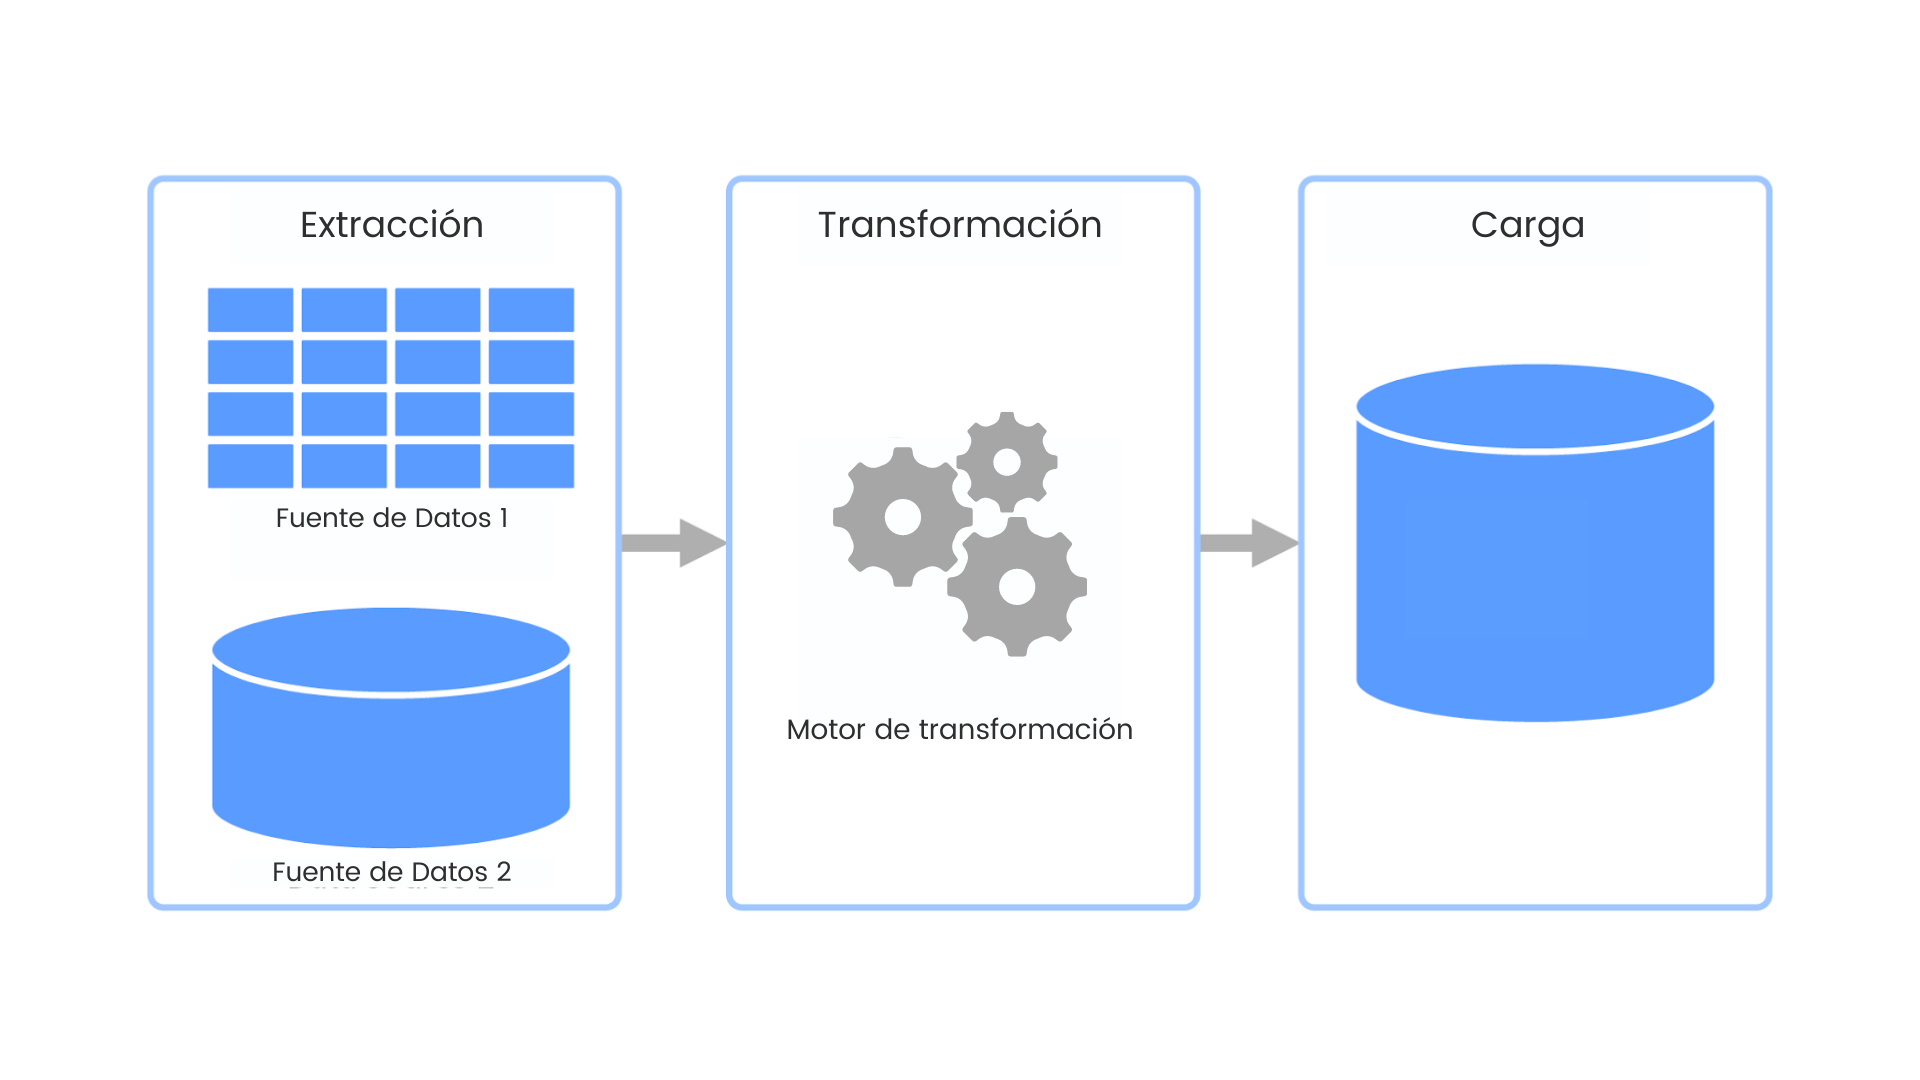
\includegraphics[width=1\linewidth]{img/etl.png}
    \caption{Estructura de un proceso ETL}
    \label{fig:ProcesoETL}\cite{ProcesoETL} 
\end{figure}

\paragraph{Transformación de Datos:}
en esta segunda fase los datos van a ser transformados y limpiados, ya que las herrmaientas que pertenecen a esta parte del proceso ETL permiten: cargar solo ciertas secciones o columnas, modificar tipos de variables, agrupar los datos en rangos preseleccionados o generar nuevos campos a partir de los existentes.

\paragraph{Carga de Datos:}
en la última parte del proceso consiste en que una vez tengamos los datos transformados, estos vayan siendo cargados en el lugar destino que le indiquemos (e.g., ElasticSearch) para que allí sean indexados y gestionados de una manera concreta.
